\chapter{Implementation}%%%%%%%%%%%%%%%%%%%%%%%%%%%%%%%%%%%%%%%%%%%%%% 
\label{chap:implementation}
This chapter presents the implementation of the methodology. 
% an implementation of this design
It discusses the extent of the achieved functionality, as well as certain ways it fell short of the proposed design.

\section{Introducing: Geofront}
\label{sec:implementation:app}

\begin{note}
  
\end{note}

\begin{figure}
  \centering
  \graphicspath{ {../../assets/images/implementation/} }
  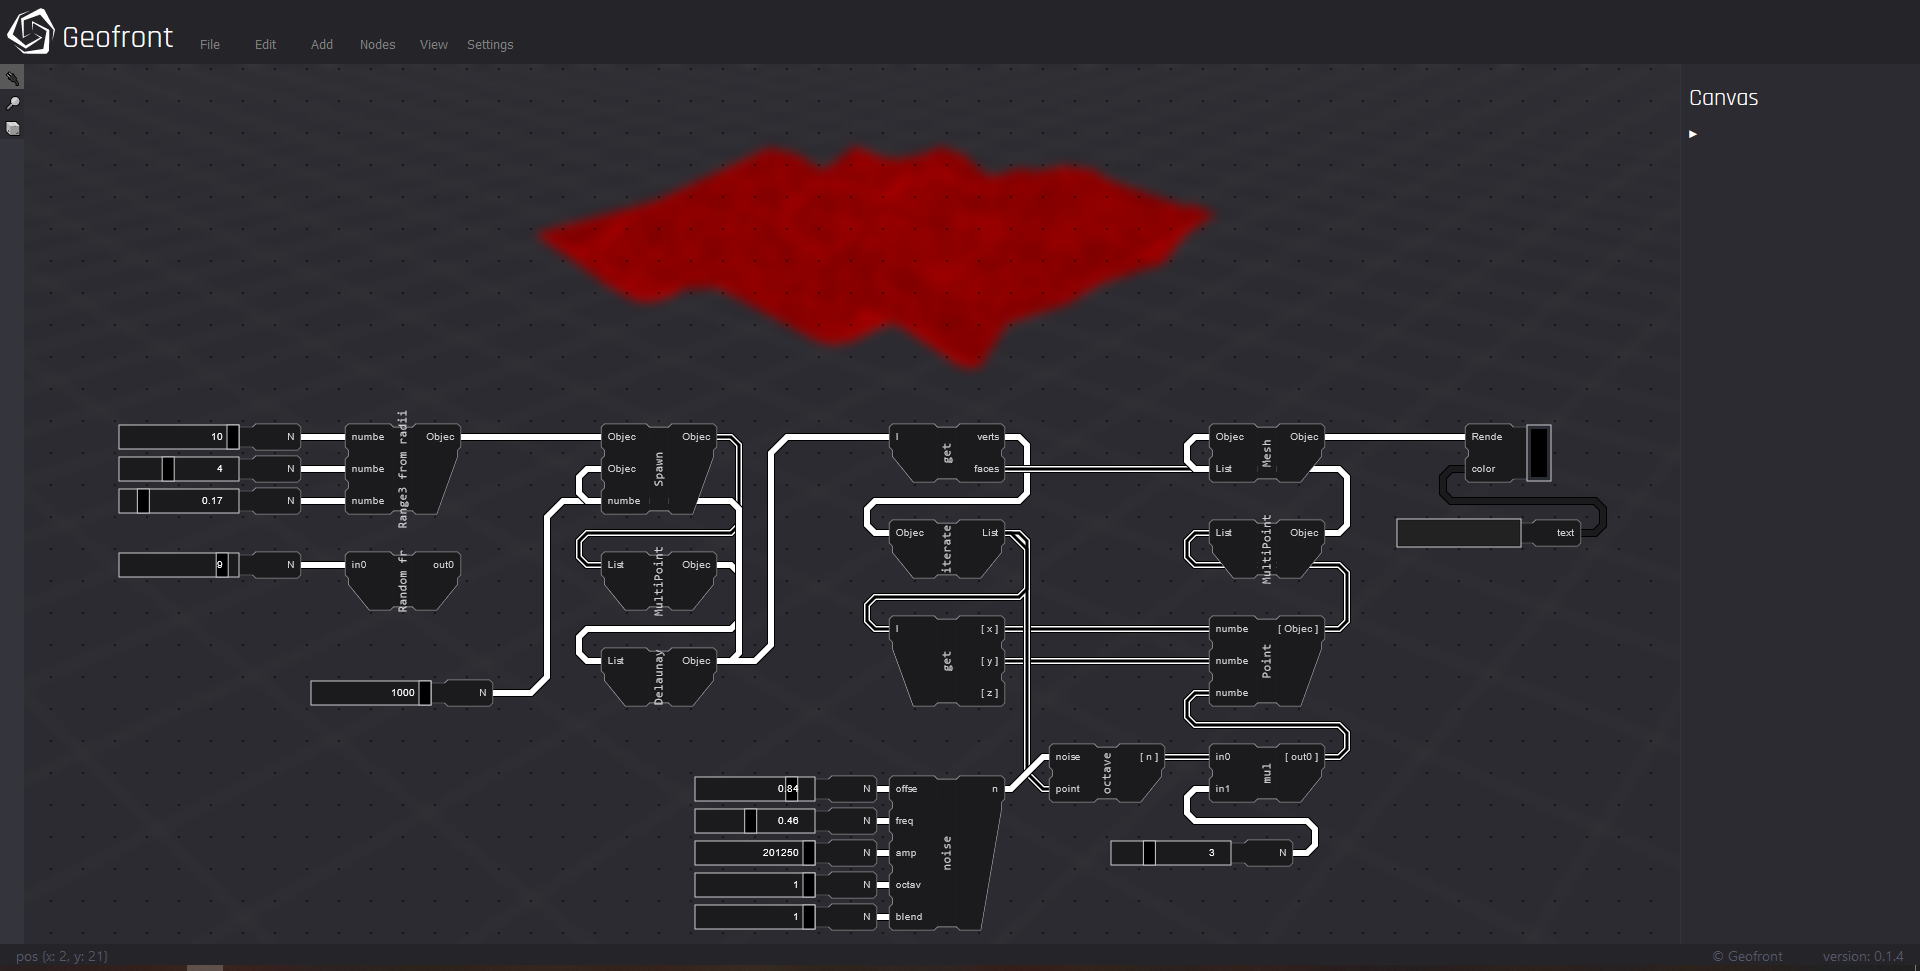
\includegraphics[width=\linewidth]{full-application.png}
  \caption[Geofront]{The Geofront Application}
  \label{fig:geofront-app}
\end{figure}

This section discusses the extent of the prototype \ac{VPL} implementation. 
The prototype is titled "Geofront", as a concatenation of "geometry" and "frontend".
Geofront exists as a set of loosely coupled repositories, all published on the version control platform GitHub under the MIT license. These repositories are grouped under the GitHub Organization \m{thegeofront} .

% TODO: do something with appendix
% (SOURCE: https://github.com/thegeofront)

The Geofront Application is implemented according to the design layed out in \refsec{sec:method:base-vpl}, and uses TypeScript as its main language. 
\m{webpack} is used to compile this codebase into a singular JavaScript file, and this file practically serves as the full application. 
the repository spend around 9.000 lines of code, divided into core categories and functionalities.
What follows is a clarification of the implementation of some of these categories.

% TODO make this!!!!
% \subsection{Framework}

% ...

% ... 

\subsection{Model}

The visual programming language model as described by \refsec{sec:method-model} and \reffig{fig:geofront-uml} could be fully implemented on the web. 
Both the shims as well as the model itself was implemented in TypeScript (TS). 
This model allows Geofront to internally represent the data structure and logic of a dataflow-VPL program. 

Type safety was fully implemented by essentially creating a new 'layer' of hierarchal types on top of TS / JS, as proposed by the methodology.

The type system can be extended by types found in third party Plugins.  
In theory, this can be used to prevent all incorrect type usage during creation of a Geofront graph, and before calculation.
In practice, to support iteration, some runtime type checking was still required. 
Additionally, the type system had to be disabled in situations were plugins did not produce interface types (such as projects compiled using emscripten).

\subsection{View}

\subsubsection{The graph}

\begin{figure}
  \centering
  \begin{subfigure}[b]{0.30\linewidth}
    \graphicspath{ {../../assets/images/implementation/} }
    \centering
    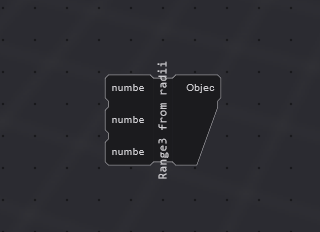
\includegraphics[width=\linewidth]{node.png}
    \caption{}\label{fig:node-cable:1}
  \end{subfigure}%
  \qquad 
  \begin{subfigure}[b]{0.30\linewidth}
    \graphicspath{ {../../assets/images/implementation/} }
    \centering
    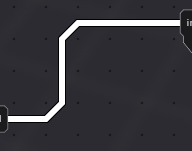
\includegraphics[width=\linewidth]{cable.png}
    \caption{}\label{fig:node-cable:2}
  \end{subfigure}%
  \qquad 
  \begin{subfigure}[b]{0.30\linewidth}
    \graphicspath{ {../../assets/images/implementation/} }
    \centering
    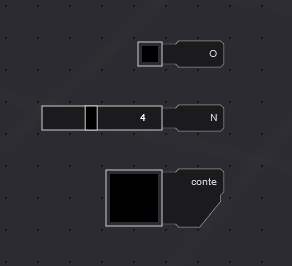
\includegraphics[width=\linewidth]{widgets.png}
    \caption{}\label{fig:node-cable:3}
  \end{subfigure}%
  \caption{The basic canvas components of Geofront: a Node (A), a Cable (B), and multiple Widgets (C) }
  \label{fig:node-cable}
\end{figure}

The graph data model must be rendered to the screen so users can comprehend and edit the graph. 
This visualization is achieved by using the HTML5 Canvas Api. 
The Canvas API is a raster-based drawing tool, offering an easy to use, high-level api to draw 2D shapes such as lines, squares, circles, and polygons. 
The Nodes Canvas uses this API to draw polylines and polygons at runtime, to represent the cables and nodes respectively. 
These basic shapes and their styles change dynamically, based on features like the length of a cable, how many input sockets a node requires, or whether or not a node is selected. 

Like other HTML5 features, the main advantage is that this API is included and implemented within the browser itself. This method is fast thanks to its C++ based implementation, and can be used without the need to include anything within the source code of the application.

Additionally, the Canvas API provided granular control over how and when shapes should be rendered. 
This feature was instrumental in providing Geofront with a wide range of widgets, containing sliders, text fields, image viewers, file load, fetch, and save widgets, and even a component capable of opening up third-party applications as a pop-up (\reffig{fig:node-cable:3}). 

The downside of this implementation, is that all features the HTML renderer normally accounts for, like picking, conditional styling, and performant rendering of repetitious elements, are lost.
These had to be re-implemented in typescript, which will never be as performant as the codebase of the browser engines themselves. 
An additional limitation is that the draw calls are primarily CPU based, 
making it less performant than a pure WebGL implementation would have been.
lastly, the implementation chose to redraw the full canvas on every registered change to the graph, instead of partial redraws. 

These limitations come together to a performance linear to the amount of nodes and cables drawn. For the current implementation and scale of Geofront, this performance is acceptable.  
Still, the application slows down when rendering a large amount of components. 

% \begin{note}
%   TODO Show a graph with performance considerations
% \end{note}


% \begin{note}
%   TODO Show a table with all GUI nodes!!
% \end{note}

This performance hit is partially due to the implementation, and partially due to browser feature limitations. 
The browser does not offer a 'middle ground' between html-like rendering and 2D canvas-like rendering required for a visualization like the dataflow graph. 
Still, this implementation could have experimented more with a HTML + SVG based render method.

\subsubsection*{Presentation}

\begin{figure}
  \centering
  \graphicspath{ {../../assets/images/implementation/} }
  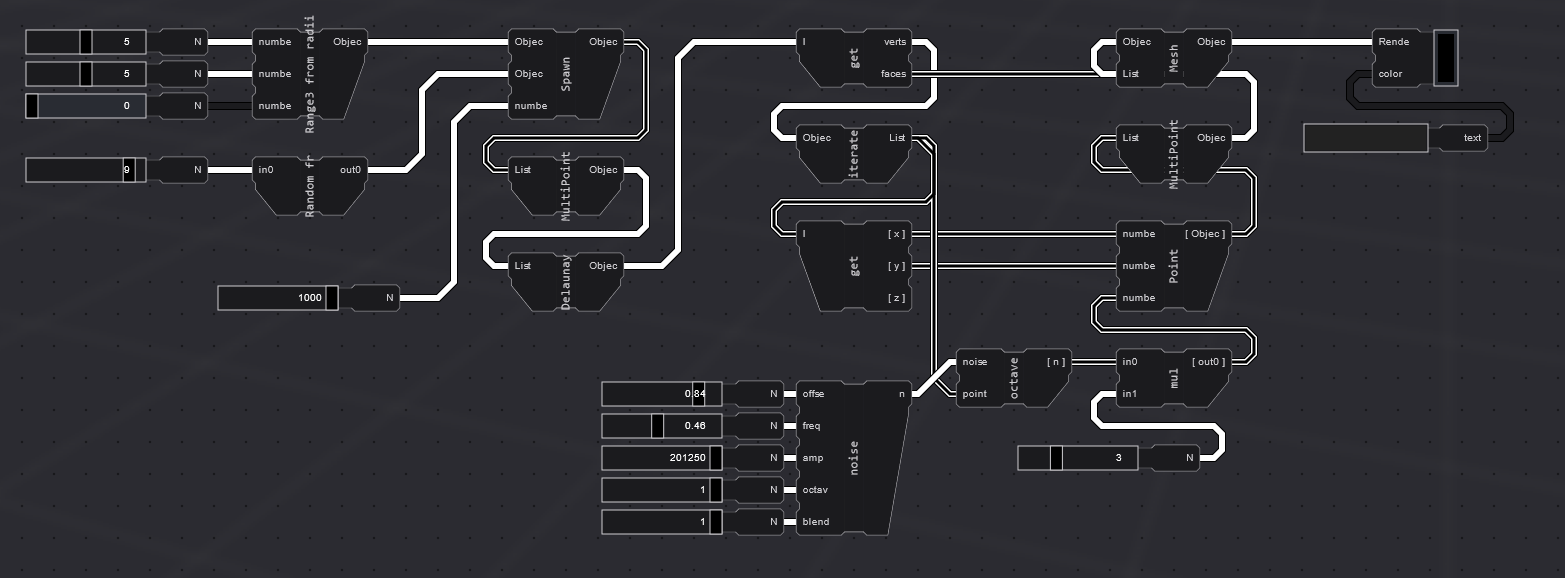
\includegraphics[width=\linewidth]{a-full-graph.png}
  \caption[Shim Classes]{A complete Geofront script}
  \label{fig:a-full-graph}
\end{figure}

Special care has been put into the presentation of the implementation.
The layout takes inspiration from various geometry VPLs mentioned at \refsec{sec:related-geovpl}, such as Blender's GeometryNodes, McNeel's Grasshopper, and Ravi Peter's GeoFlow. 
A few notable exceptions, however. 
Firstly, the entire graph is placed on a grid, and all nodes adhere to this grid (see \reffig{fig:a-full-graph}). 
For example, a node with three inputs will always occupy three grid cells in height. 
This grid is applied for much of the same reason as terminals \& source code are displayed using monospaced fonts. 
Consistent sizing encourages organization and clarity, for this makes it easy for components to line up, and predict how much space something requires.  
Cables also adhere to the grid. They alter their shape in such a way to remain as octagonal as possible, in an attempt to make connections between nodes more readable.
% This takes some additional inspiration from subway maps, as well as the design of computer chips. 
% This makes for a good fit, as these spatial configurations and the Geofront Script are all focussed on organizing connectivity.

\subsubsection*{3D Viewer}

\begin{figure}
  \centering
  \graphicspath{ {../../assets/images/implementation/} }
  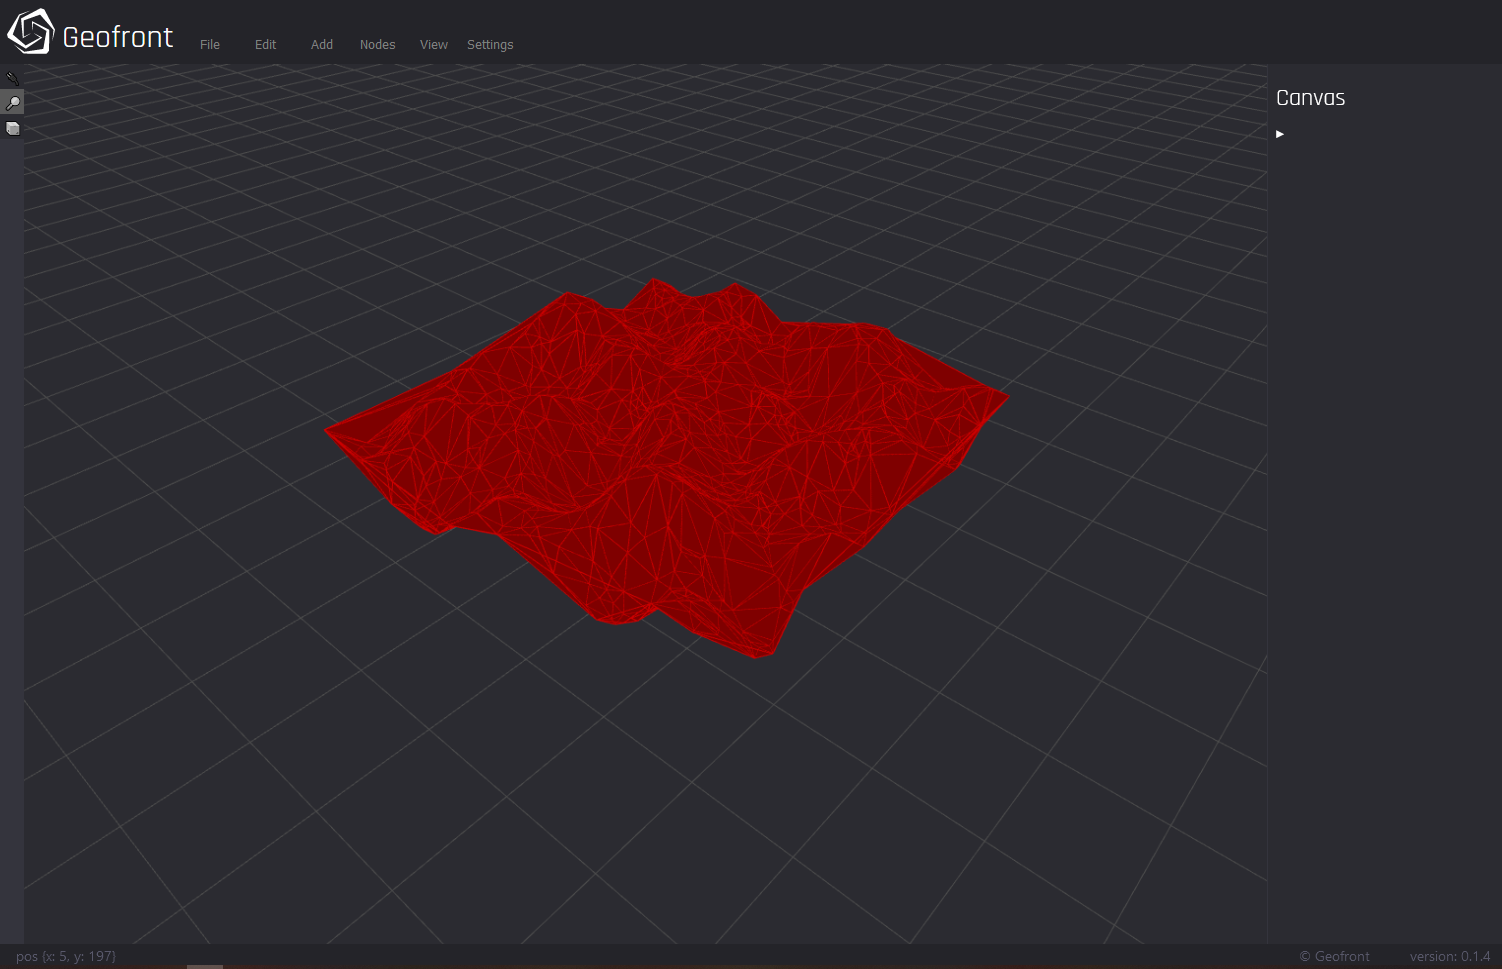
\includegraphics[width=\linewidth]{viewer.png}
  \caption[Geofront viewer]{The Geofront Viewer}
  \label{fig:geofront-viewer}
\end{figure}

The 3D viewer attached to the geofront application is also implemented in typescript. 
It uses WebGL and the OpenGL Shading Language (glsl) as its graphics API. 
The viewer can be used to represent and visualize various geometries, such as points, lines, meshes, bezier curves, and bezier surfaces.
Images can also be rendered, which are represented as a quad mesh with a texture. 

The useful aspect of WebGL is the fact it does not have to be included within the source code of a program. 
WebGL supports all render demands basic, small-scale 3D geodata visualization might need, such as point clouds and DTMs.
large scale visualization is not possible, as the visualizer does not support idioms like frustum culling, or dynamic levels of detail. 
Additionally, the viewer does not support

These visualization options open the possibility of visualizing a great number of different geodata types, such as DTM / DSM, GEOtiff, Point clouds, and OGC vector data. 
However, specific visualization convertors are not implemented, for these are reliant upon the compilation of existing geocomputation libraries. 

\begin{figure}
  \centering
  \begin{subfigure}[b]{0.45\linewidth}
    \graphicspath{ {../../assets/images/implementation/} }
    \centering
    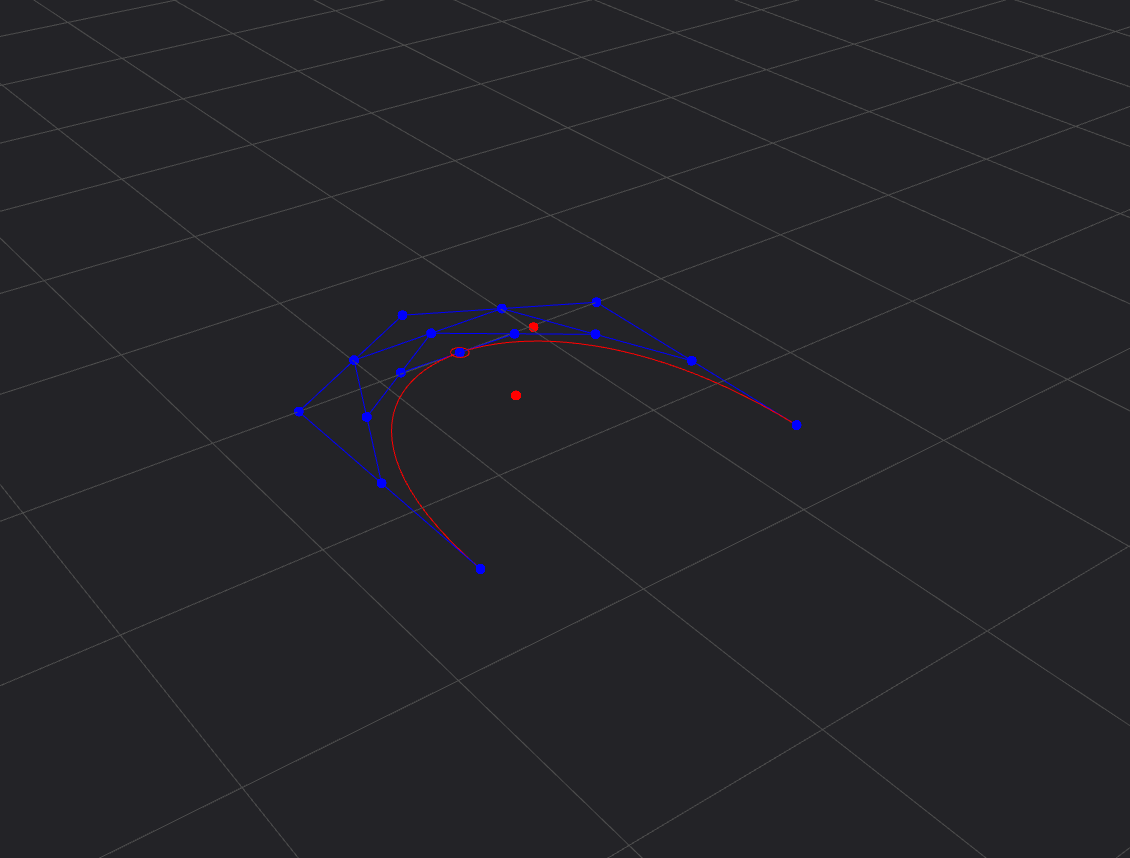
\includegraphics[width=\linewidth]{viewer-2.png}
    \caption{}\label{fig:viewer-geometries:1}
  \end{subfigure}%
  \qquad 
  \begin{subfigure}[b]{0.45\linewidth}
    \graphicspath{ {../../assets/images/implementation/} }
    \centering
    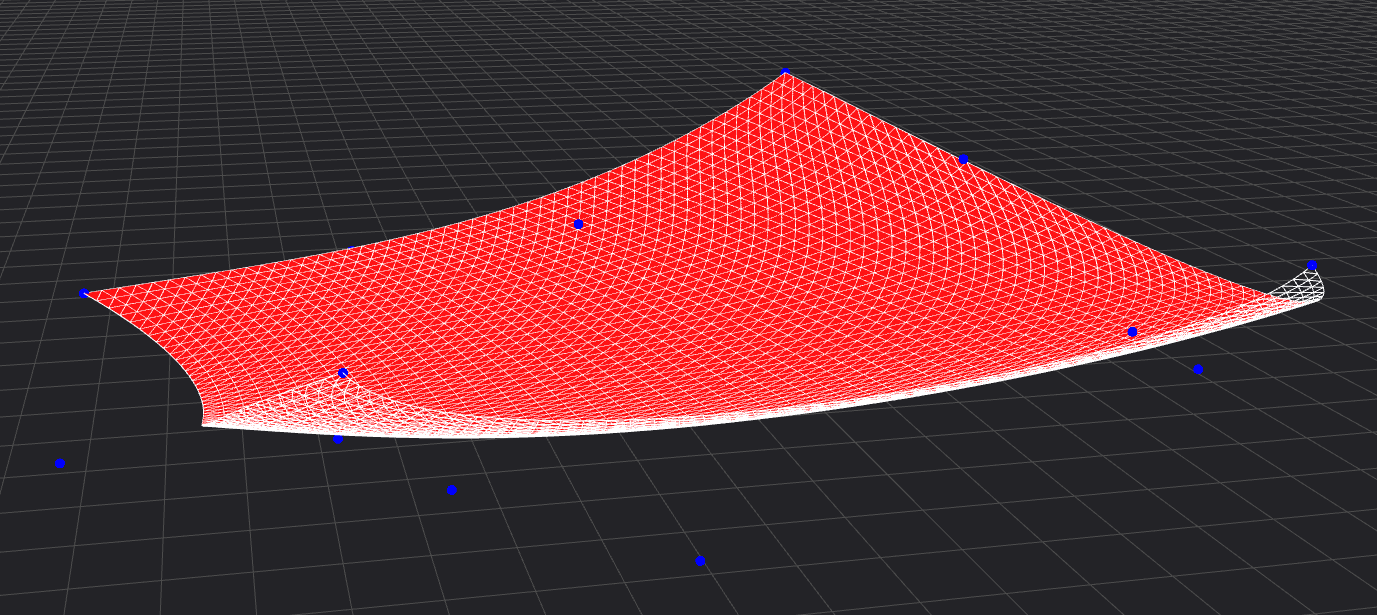
\includegraphics[width=\linewidth]{viewer-3.png}
    \caption{}\label{fig:viewer-geometries:2}
  \end{subfigure}%
  \caption[Geofront viewer geometries]{A bezier curve and surface visualized using the geofront viewer}
  \label{fig:viewer-geometries}
\end{figure}

\subsection{Controller}

% \item an interface to create and edit this graph 
% \item a way to provide input data 
% \item a way to execute the language
% \item a way to display or save output data

% \subsubsection*{Calculation}
% Execution of the graph is implemented as described by the methodology, albeit with a major setback: execution does not run on a separate thread. 
% This means that the interface freezes up during large calculations.

% The reason for this is the difficulty in achieving concurrency in the browser. 
% Web workers have to be implemented and instantiated using separate JavaScript files. 
% Not only is this unusual, it forces a codebase to create separate files per multithreaded operation.
% The dynamic nature in which some of Geofront dependencies are loaded made splitting up the codebase like this difficult, let alone using multiple threads for calculating each node.

% Additionally, both Typescript and WebAssembly do not make the mutability of variables explicit, nor was this implementation able to find a substitute method to add a mutability model on top of these languages. 
% This made implementing the concurrency model explained in \refsec{sec:method-controller} impossible.

\subsubsection{Interaction}
User interaction is made possible through the HTML DOM Events. 
This API provides ways to listen to many events, including keyboard and mouse events. 
When the mouse is moved, its screen-space position is transformed to a grid position, which allows the user to select one or multiple objects. 

Geofront's user interface aims to mimic features of regular desktop applications. 
As such, the Geofront Graph supports features like undoing, redoing, duplication, copying, and pasting. 
These functionalities can be used with the expected keyboard combinations (Ctrl + C / Ctrl + V).
However, the implementation does lack touch \& mobile support.

In general, these editing features are complete, but there are a few caveats caused by the browser environment.
Namely, the browser has need of its own controls and shortcuts. 
For example, the right mouse button brings up the browser context, and the \m{Ctrl + W} shortcut closes a browser tab, which cannot be overwritten.
While there are some workarounds, these aspects make it so Geofront, and web applications mimicking desktop applications in general, may behave unexpectedly.

\subsubsection*{Input and Output}
The base dataflow VPl component of Geofront support input and output UI elements, like sliders, buttons, and text fields.
These form special nodes on the canvas, called 'widgets'. 
Widgets simply are nodes with side effects. 
By making this a different type of node, the behavior of the graph becomes more predictable.

The fact that the Geofront implementation opted for a canvas API-based visualization made it so HTML could not be used for these aspects, and all these features had to be created within the constraints of the Canvas API.

Files can be used as inputs and extracted as outputs using the 'file load' and 'file save' widgets. 
These files are then loaded as raw text or raw binary, which can be parsed by using a parser appropriate for that file type. 
The problem with this implementation, is that it requires a full file to be loaded into memory. 
Most native parsers make use of streaming to avoid this. 
There are ways of supporting incrementally reading files in a browser, but these methods are not supported by all browsers yet. 

%%%%%%%%%%%%%%%%%%%%%%%%%%%%%%%%%%%%%%%%%%%%%%%%%%%
%%%%%%%%%%%%%%%%%%%%%%%%%%%%%%%%%%%%%%%%%%%%%%%%%%%
%%%%%%%%%%%%%%%%%%%%%%%%%%%%%%%%%%%%%%%%%%%%%%%%%%%


\newpage
\section{The plugin system}
\label{sec:implementation:loading}

The plugin system is implemented according to design discussed in \refsec{sec:method:plugin-system}.
The implementation comes down to a plugin loader written inside of the Geofront application, with an accompanied workflow of how to create such a plugin. 

\subsection{The plugin loader}
\label{sec:implementation:loading:limits}

The plugin loader implemented in Geofront can load a JavaScript / typescript library, and convert it into appropriate visual components. 

As prescribed by the methodology, Typescript declaration files are loaded to determine the name, location, parameter types of functions. 
This works similar for libraries which include a WebAssembly binary.

While in theory any JavaScript / typescript library can be used, in practice some limitations are in place due to the specific implementation used:

\subsubsection*{Files}
Firstly, the current loader accepts only one Javascript file, and one Typescript Declaration file per library.
A library without a 'd.ts' declaration cannot be used. 
If additional files are used, such as \ac{wasm} files, these will have to be explicitly fetched and run by the JavaScript file. 
For the purposes of this study this is acceptable, as the used \ac{wasm} compilers work in a manner compatible to these limitations.
Javascript bundlers also help to adhere to these limitations.
Still, this does mean that not just any JavaScript library can be imported. 

\subsubsection*{Library Structure}
Secondly, while the loader does support namespaces and classes, not all types of libraries and programming styles are supported. 
Functions using callbacks, promises, complex types, or generics, cannot be properly loaded. 
Libraries utilizing "method chaining APIs" can be loaded, but are difficult to use as intended on the Geofront Canvas.
% Also bear in mind that the loader does not perform any checks to see if the loaded library actually uses pure functions. 

\subsubsection*{Types}
The plugin loader can only load functions using acceptable input and output types. 
Not all input and output arguments translate well to the format of a dataflow VPL. 
The types may only include: 
\begin{itemize}
  \item basic JavaScript types (boolean / number / string)
  \item basic jsons (unnamed structs), objects, interfaces 
  \item JavaScript ArrayBuffers like \m{Float32Array} (vital for performant data transfer)
\end{itemize}
The typesystem of the plugin loader will pick up on types exposed by a library, and include them within the type safety system of Geofront. 
However, this does mean that certain types are not supported, like asynchronous promises, or functions as variables. 

% \begin{figure}
%   \centering
%   \graphicspath{ {../../assets/diagrams/} }
%   % 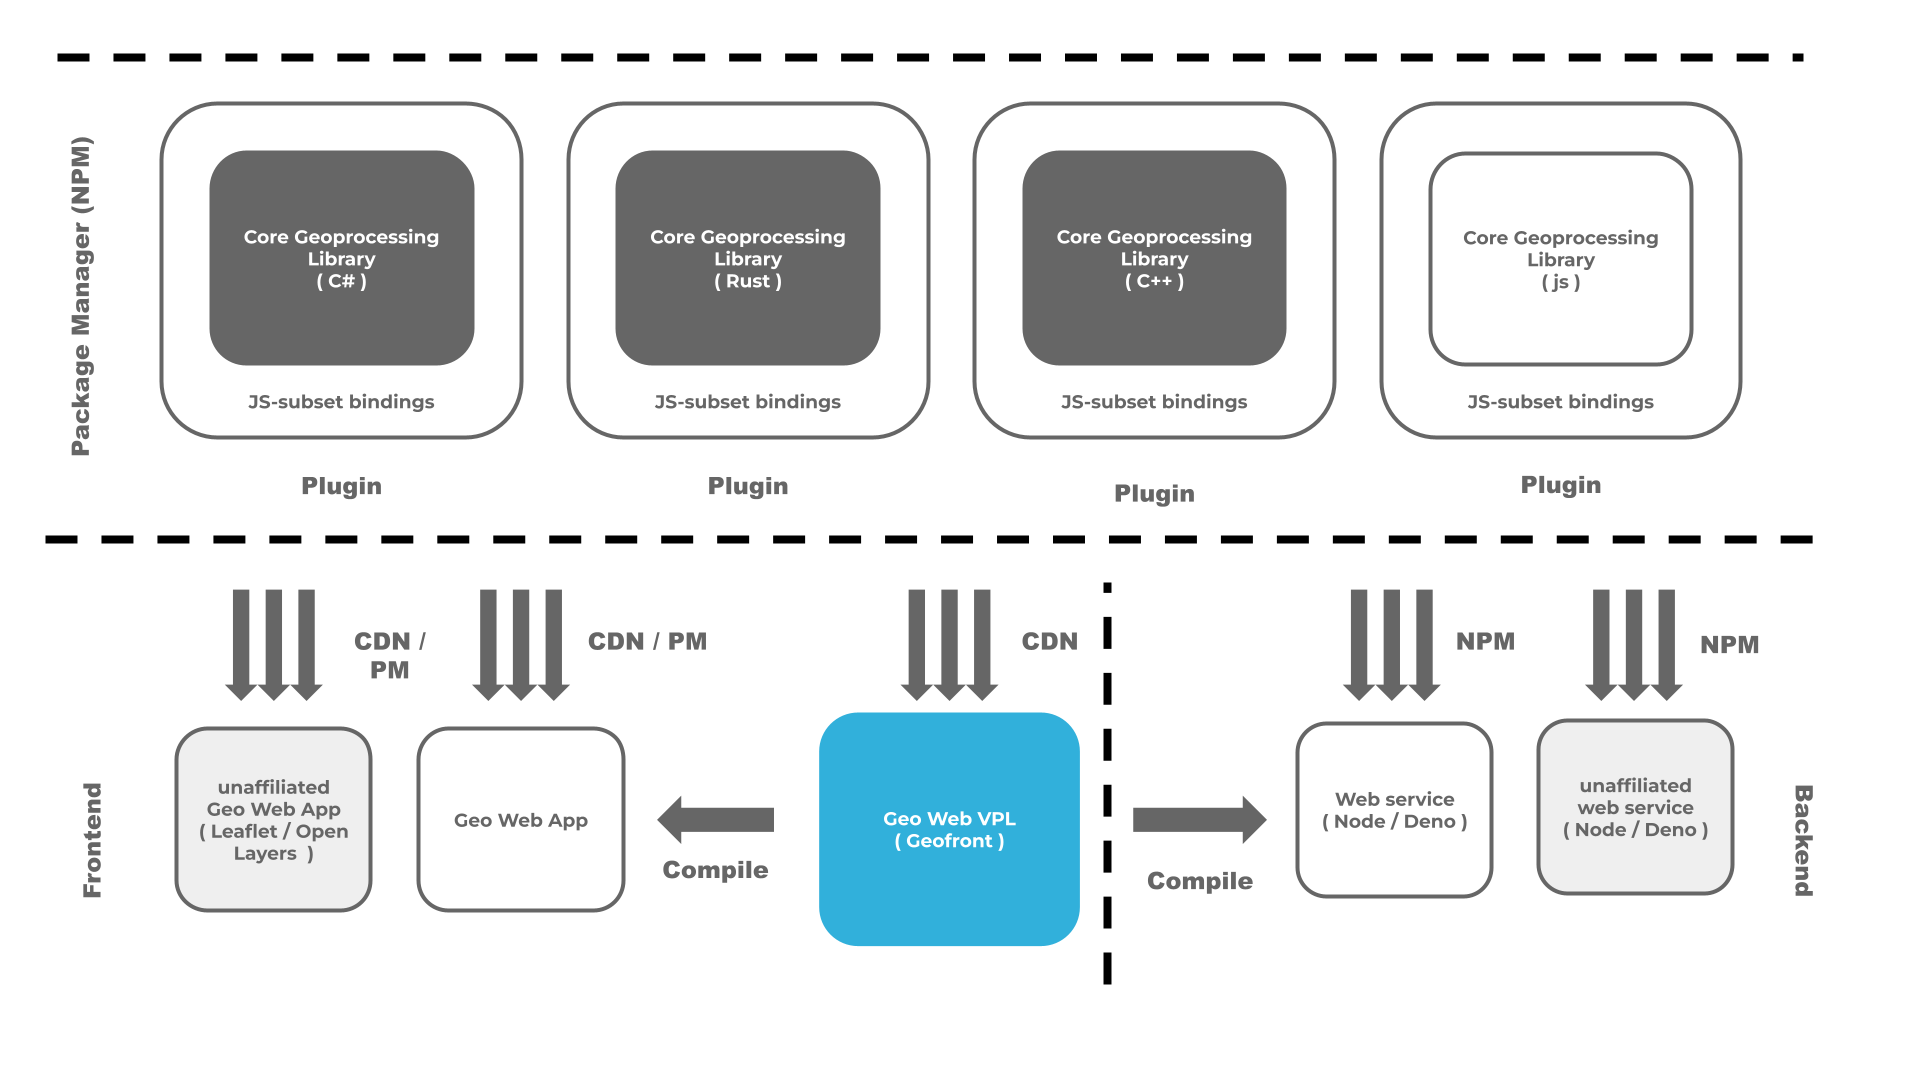
\includegraphics[width=\linewidth]{Model Proposal.png}
%   \caption[]{TODO: show importer side-by-side}
%   \label{fig:todo-1}
% \end{figure}


% \begin{figure}
%   \centering
%   \graphicspath{ {../../assets/diagrams/} }
%   % 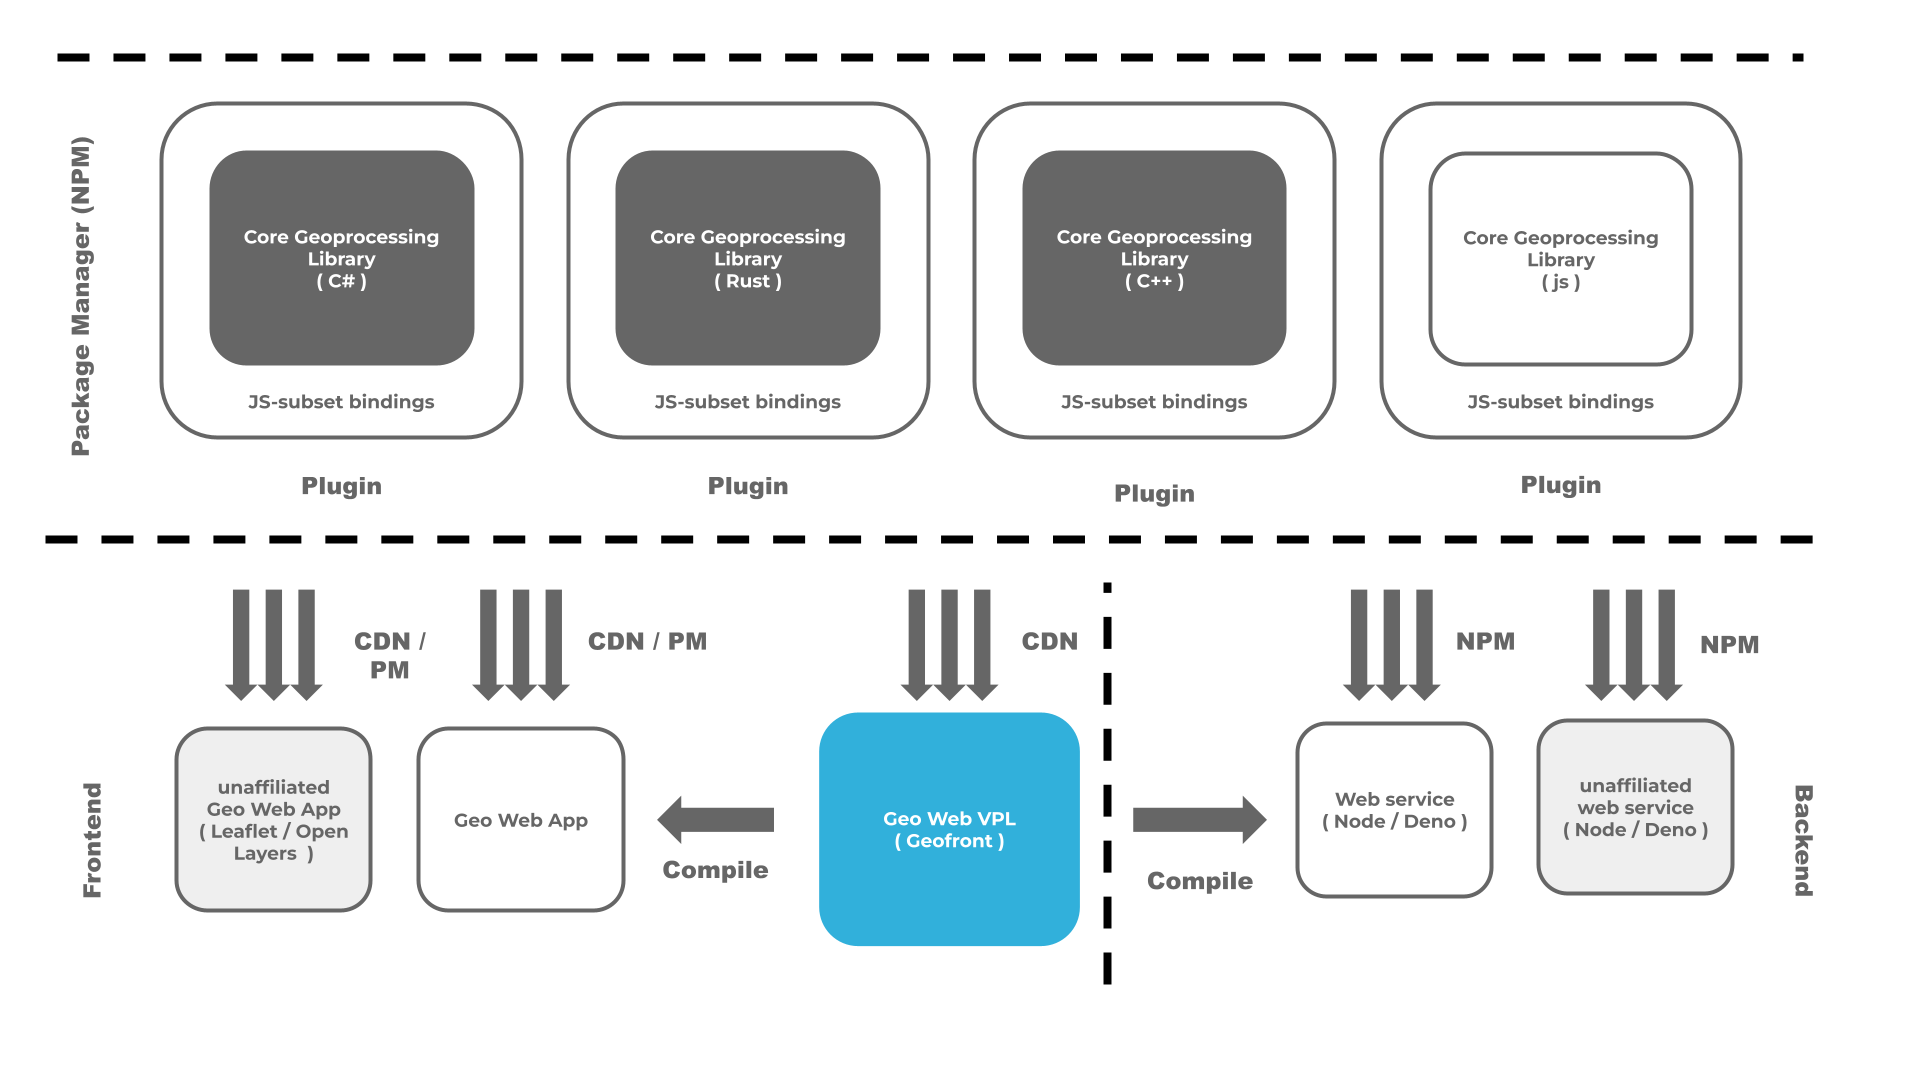
\includegraphics[width=\linewidth]{Model Proposal.png}
%   \caption[]{TODO: show more achieved functionality}
%   \label{fig:todo-2}
% \end{figure}

\subsubsection*{Supported languages}
Finally, not all languages are equally supported:

\begin{itemize}[-]
  \item \textbf{Javascript / Typescript}: 
    If the Javascript and Typescript files used adhere to the limitations mentioned above, the library can be used. 
    However, a bundler needs to be used to include all sub-dependencies of a library, as the Geofront loader does not load sub-dependencies currently. 

  \item \textbf{Rust}:
    Libraries compiled to webassembly using the "\m{wasm-bindgen}" work "out of the box" in most cases.
    \m{wasm-bindgen} is able to generate JavaScript wrapper bindings for a \ac{wasm} library, accompanied by TypeScript type definitions. 
    This wrapper handles type conversions. 
    
    However, rust libraries compiled to the web do require a initialization step. 
    As such, the loader now checks if the library looks like a Rust library, and if it does, it uses a slightly altered loading method.
  \item \textbf{C++}
    At the time of writing this study, the 'embind' compiler (explained in \refsec{sec:implementation:loading}) does not have an option to compile a typescript declaration file. 
    Additionally, the JavaScript generated to wrap the wasm binary is not a wrapper handling type conversions and memory safety like Rust. 
    Instead, it uses a custom architecture programmatically expose JavaScript wrapper functions one by one, and leaves it to the user of the library to deal with type conversions and memory safety. 
    These two aspects combined makes it so C++ cannot use Geofront's loader directly, and must use an additional in-between wrapper libraries.

  \item \textbf{Other languages}
    This study only experimented with Rust and C++ as non-js languages.
    While the loader's ability to work with WebAssembly is promising, additional testing is required before Geofront can claim to support any language. 
\end{itemize}

\subsection{Achieved Workflow}
\label{sec:implementation:workflow}

% \emph{show the insane (rust + wasm + npm) workflow}

With all the above considerations in mind, the following workflow can now be used to create a Geofront Plugin, which, as explained, doubles as a normal JavaScript library. 
If Rust or C++ is used, this setup in a way triples as also a native geoprocessing library.
The Geofront standard library is also implemented by using workflow with Rust.

\begin{lstlisting}
  
  Using Typescript: 
  1. Write or find a geoprocessing / analysis library 
     using typescript, 
  2. Compile and bundle to a `d.ts` + `.js` file.
  3. publish to npm 

  Using Rust: 
  1. Write or find a geoprocessing / analysis library using rust
  2. Create a second library, which exposes a subset of this 
     library as 'functions usable on the web', using 'wasm-pack' 
     and 'wasm-bindgen'.
  3. Compile to `.wasm` + `d.ts` + `.js`.
  4. publish to npm (`wasm-pack publish`)
  
  Using C++: 
  1. Write or find a C++ based geoprocessing / analysis library. 
  2. Create a second library, which exposes a subset of this 
     library as 'functions usable on the web', using 'emscripten' 
     and 'embind'.
  3. Compile to a `.wasm` and `.js` file using emscripten.
  4. Manually edit the 'js' file to wrap initialization and type conversions.
  5. Manually create a corresponding `d.ts` file, calling newly created methods in the 'js' file.
  6. Publish these to npm 

  ---------------------------------------------------------

  In Geofront: 
  A. Reference the CDN (content delivery network) address of this node package. 
  B. Use the library.

\end{lstlisting}

% \begin{figure}
%   \centering
%   \graphicspath{ {../../assets/diagrams/} }
%   % 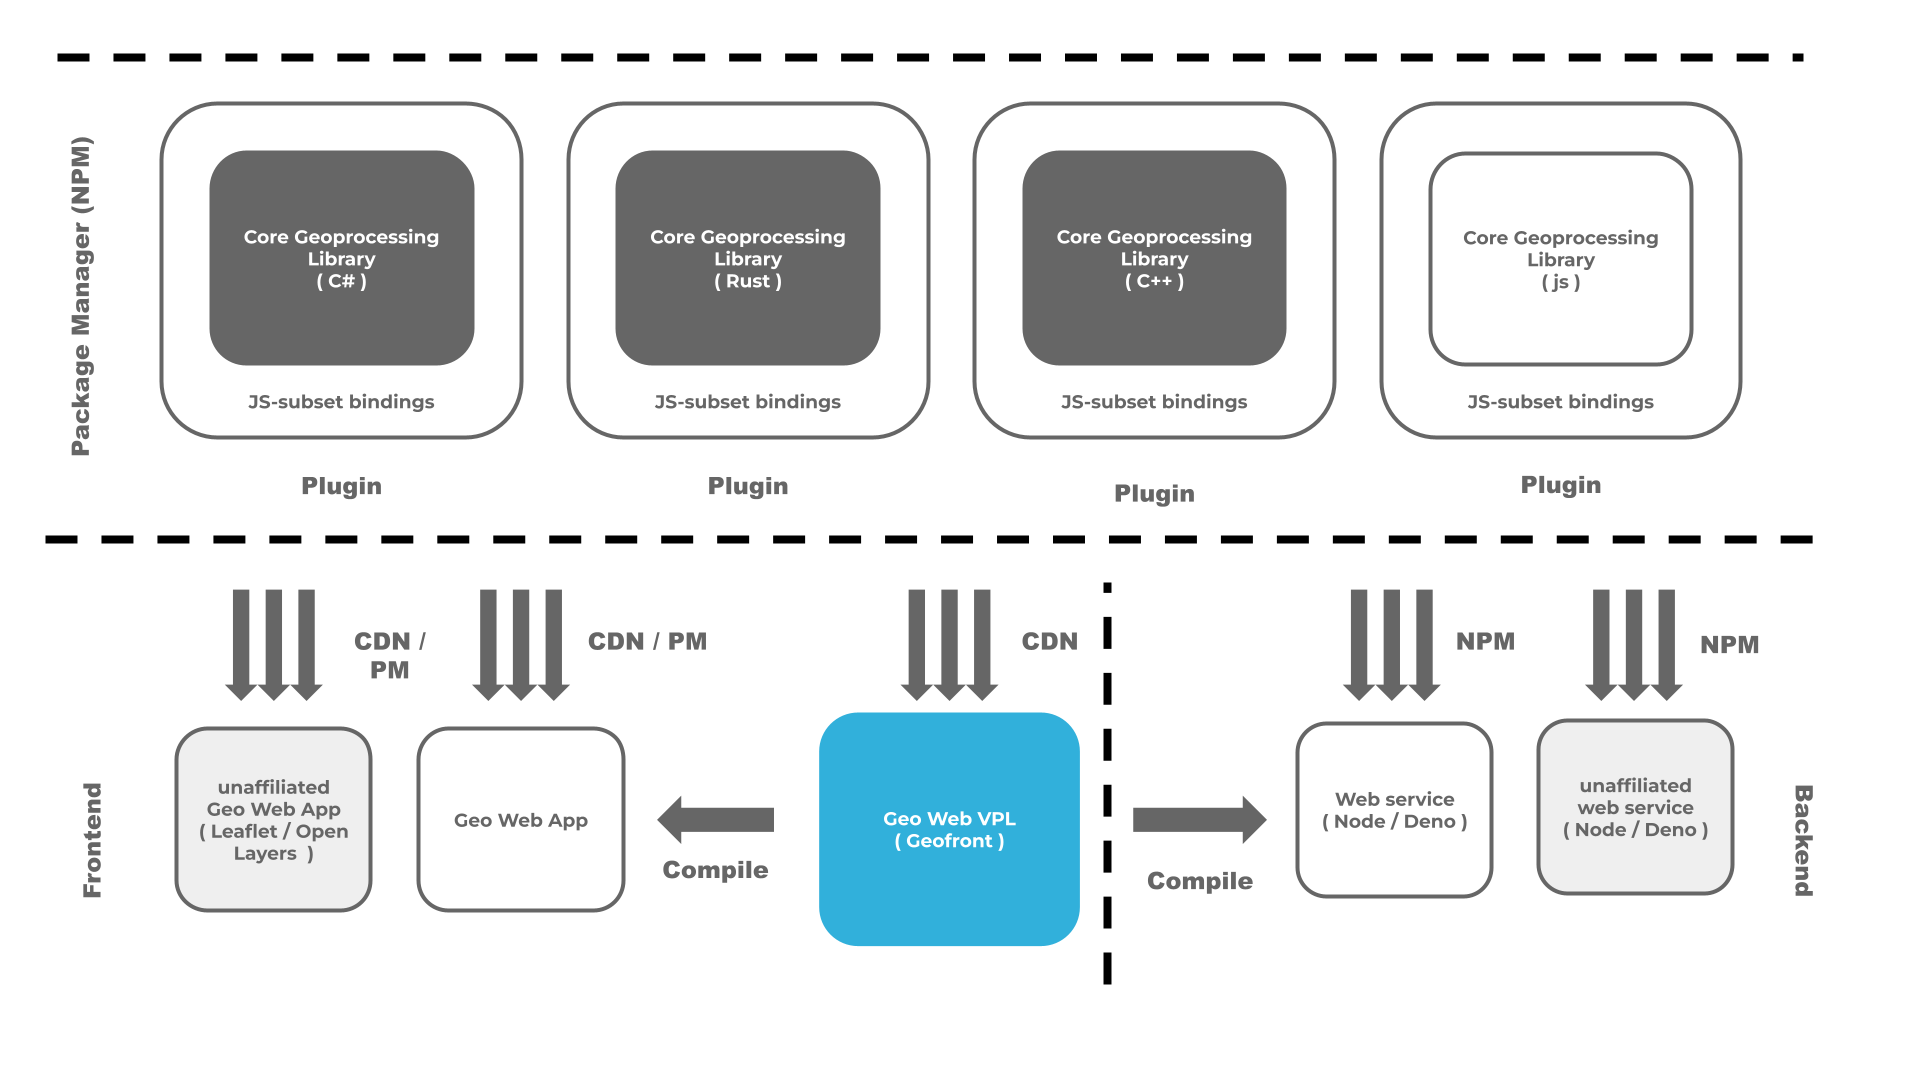
\includegraphics[width=\linewidth]{Model Proposal.png}
%   \caption[]{TODO: show the achieved workflow visually}
%   \label{fig:todo-more-images}
% \end{figure}

\subsection{Automation and portability}

The \refsec{sec:method:plugin-system} mentioned the requirements of library portability and automation. 
In this section we assess to what extent this implementation was able to succeed on delivering these two requirements. 

\subsubsection*{Automation \& exposure of metadata}

Based on the results, we can state that the loader mitigates the need for explicit configuration only for the required, mandatory aspects. 
All optional properties like human-readable names and descriptions, must be specified explicitly using a naming convention specific to Geofront. 

In practice, however, there are some more "configuration" requirements. 
The limitations outlined by \refsec{sec:implementation:loading:limits} show that there are quite a few additional considerations. 
Geofront does not support all types or all library structures, and certain languages require additional compile limitations.

Also, while the optional properties are just that, optional, one could argue that some of these properties are in fact required. 
Libraries without 'human-readable' names and descriptions are harder to utilize in a Geofront script by end users.
While regular programming languages also allow the creation and publication of undocumented libraries, one can question if this should also be allowed for the more end-user focussed VPL libraries.

So, while the plugin loader can load some simple textual programming libraries almost without any special configuration, sizable libraries intended for consumption by Geofront will still need to be explicitly configured for Geofront.
However, even with these requirements, this can still be considered an improvement compared to the plugin systems of geometry VPLS studied at \refsec{sec:related-geovpl}, 
in which developers are required to create a class per exposed function.

\subsubsection{Portability}

This system creates seamless interoperability between a textual programming library, and a VPL plugin to an extent. 
However, because of the reasons outlined above, it is also safe to say that this seamless interoperability is only one-directional: 
Libraries intended for consumption by Geofront double as also a 'normal' JavaScript library. 
The configuration demands of Geofront only impair the normal, JavaScript-based usage by forcing a functional style, and by including certain methods only intended for Geofront. 
Even these Geofront-specific methods might prove useful in certain scenarios, such as by providing a way to visualize data.

This seamless interoperability is less prominent in the opposite direction. 
A normal JavaScript library, or a JavaScript library using WebAssembly, can't be automatically used by Geofront in most cases. 
Most libraries use an imperative programming style, use unsupported types, or consist of multiple files.
In some cases, a library is be able to be loaded, but is then functionality impaired by the interface. 

% \begin{figure}
%   \centering
%   \graphicspath{ {../../assets/images/4/} }
%   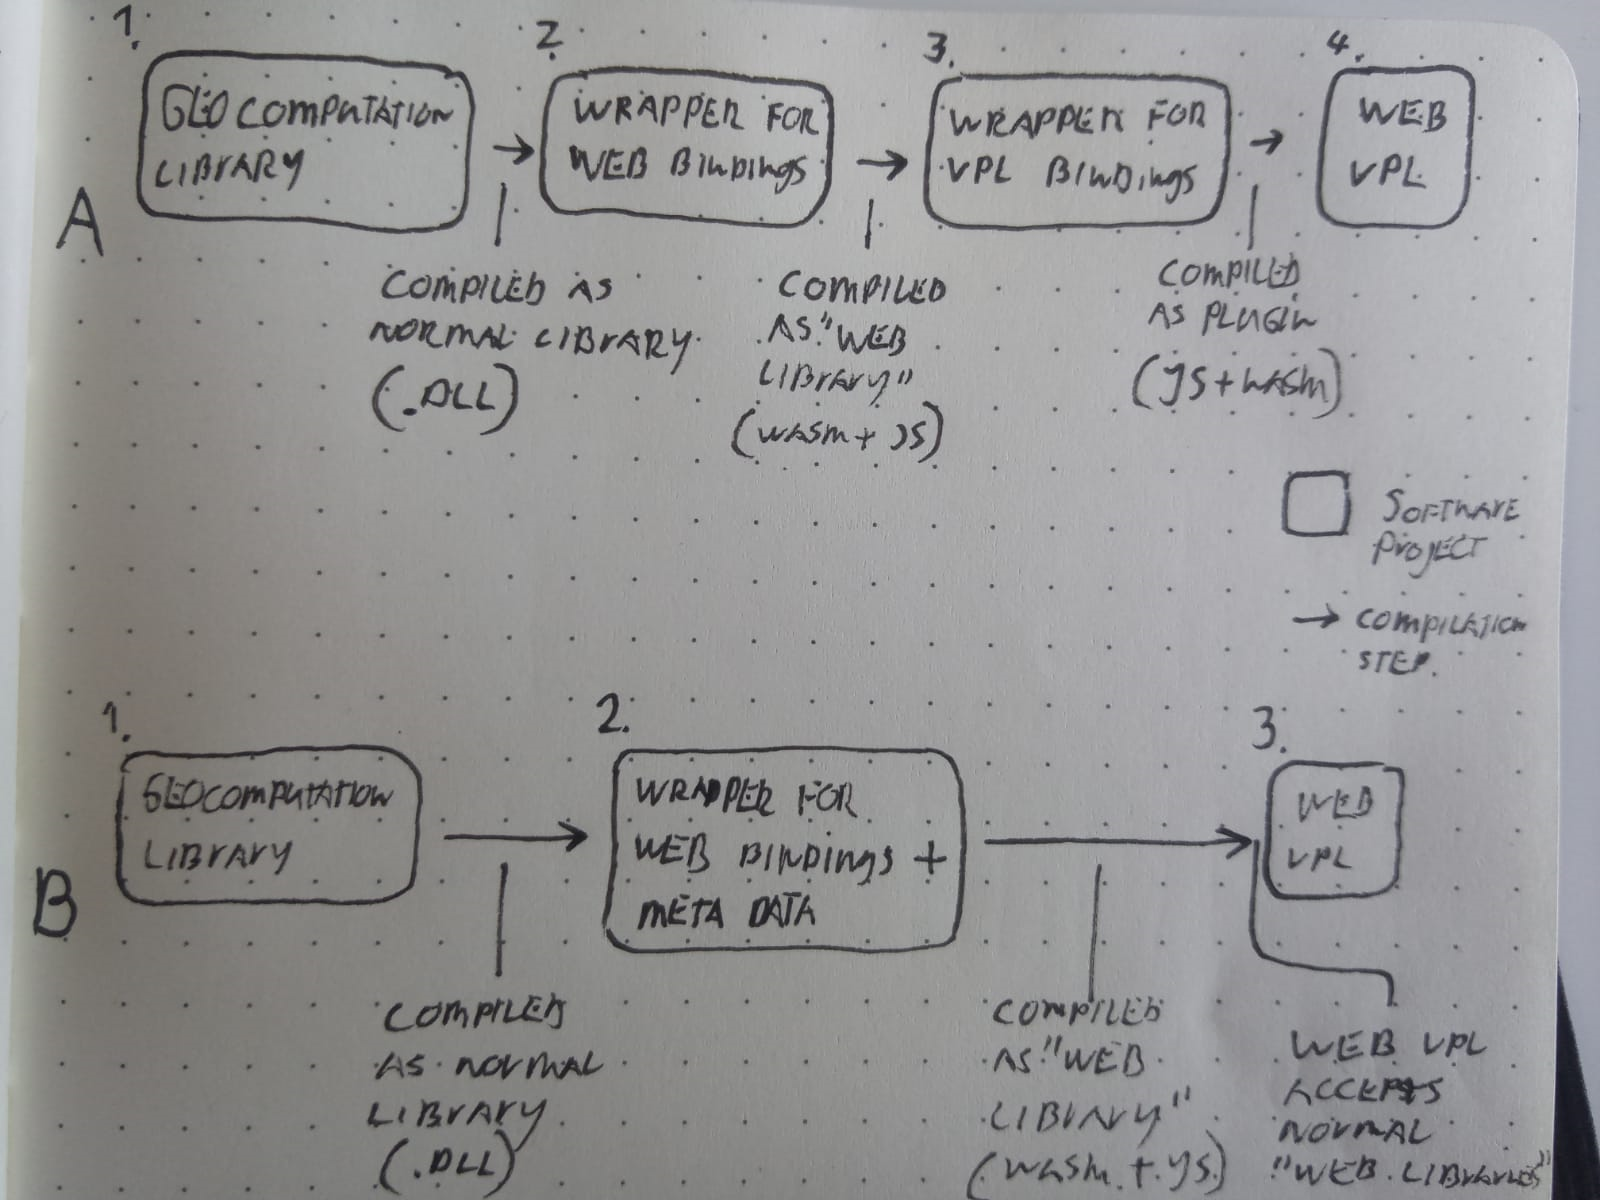
\includegraphics[width=\linewidth]{loading-trajectory.png}
%   \caption[Loading Trajectory]{Loading Trajectories}
%   \label{fig:loading-trajectory}
% \end{figure}

% \begin{note}

  % THIS IS AN ARGUMENT WHICH CAN BE USED TO DEFEND THE EFFORT TOWARDS AUTOMATION AND PORTABILITY

%   This turned out to be a problem during preliminary studies.
%   If a \ac{geo-web-vpl} wishes to use non-js libraries, it would mean that these libraries would have to be wrapped twice (see \reffig{fig:loading-trajectory} A): 
%   Once to expose the native library to the web using the methods described at \refsec{sec:method-two},
%   And once more to map the web library to the visual language. 
%   While this is a possibility, in practice, two layers of wrappers are not acceptable in terms of a development workflow.
%   This would be cumbersome, prone to errors, and hurting version control by having to synchronize between 4 software projects. 
  
%   There is also a second reason for critically addressing the way plugins are loaded. 
%   An observation was made from studying the existing geo-vpls in \refsec{sec:related-geovpl}:
%   It seems that if a developer wants to create custom VPL components, they are required to write plugins very specific to that particular VPL.
%   This means that practically, the library ecosystem of a VPL is entirely its own: 
%   It is separated from the wider context of textual programming libraries. 
%   End users are at the mercy of developers implementing their libraries in the dialect their particular VPL.
%   Meanwhile, developers are forced to implement and support a multitude of wrapper libraries for VPL platforms.  
  
%   In contrast, if the library loader of a VPL was able to directly utilize textual libraries, the barrier between VPL ecosystems and regular text-based libraries would cease to exist, benefiting both developers and end users. 
%   It might even lower the barrier between visual and textual programming in general, making it easier for VPl end-users to adopt some forms of textual programming, and vice versa. 
  
% \end{note}

\section{CLI, headless runtime}

\begin{figure}
  \centering
  \graphicspath{ {../../assets/images/implementation/} }
  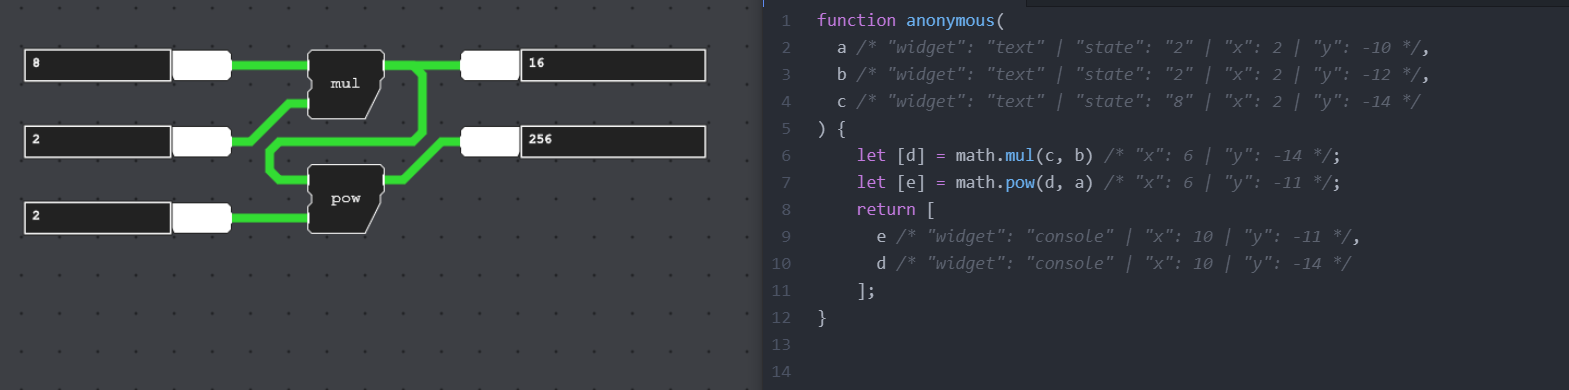
\includegraphics[width=\linewidth]{early-geofront.png}
  \caption[Geofront to js]{An early build of geofront, showcasing JavaScript interoperability }
  \label{fig:early-geofront-compile-to-js}
\end{figure}

While the zero-cost abstraction runtime, proposed in \refsec{sec:method:plugin-system}, was said not to be part of the implementation, small scale experimentation has been done as a proof of concept. 

An early build of Geofront had the ability to compile a Geofront script to a subset of regular JavaScript (see (\reffig{fig:early-geofront-compile-to-js})).  
All libraries were converted to normal import statement, all nodes were replaced by function calls, and the cables substituted by a variable token. 
Additionally, because of the no-boilerplate plugin system, this JavaScript file could be re-imported back into Geofront, to represent the exact graph it originated from. 
A subset of JavaScript was supported, using inline comments to add the appropriate metadata.
This allowed the setup shown above to be synchronized.
That is to say, updating the textual representation led to a change in the graph, and vise-versa.
This JavaScript representation could be executed headless in either a browser-based application, or using a local JavaScript runtime like Deno \citep{contributors_deno_2022}.

However, both the Pipeline to JavaScript compiler, and the JavaScript to Pipeline compiler, could not be maintained given the other requirements of the environment, such as complex \ac{GUI} nodes.
Auxiliary systems complicated the export and import workflow, like allowing a node to iterate through a list. 
Still, the brief success of the system does proof the proposed method is feasible, given enough time.